\subsection{Milestones}
Our team has decided to utilize the Agile approach for this project. We chose this methodology because it allows our team to focus on sections of the project and aligns well with the semester schedule. By making iterations for this project internally, we are able to track our progress and make status updates. Another benefit of this will be tracking any delays or problems. If we are behind on a section, we have already planned ahead and allowed ourselves room for some variance. We are also using smaller deliverables for the project which gives us more tracking because we have more internal deadlines. We will be using Jira to track our progress and add reports throughout the process. We will also be utilizing Discord as a form of communication with each other. This will be a place where we can discuss any issues or ask quick questions when we are not in person. Below, we have a high-level breakdown written for our project goals.
\subsubsection{Fall}
\begin{itemize}
    \item COMPLETED: Select components for each subsystem
    \begin{itemize}
        \item Document selection reasoning
        \item Order to ensure on-time delivery
    \end{itemize}
    \item Model physical bed
    \begin{itemize}
        \item This item was not completed and will be added to Spring
    \end{itemize}
    \item Build physical bed
    \begin{itemize}
        \item This item was not completed and will be added to Spring
    \end{itemize}
    \item PARTIALLY COMPLETED: Understand how subsystems will integrate:
    \begin{itemize}
        \item Communication protocols (REST, I2C, SPI, DSP, etc)
        \item Power requirements
    \end{itemize}
    \item UI for Web subsystem
    \begin{itemize}
        \item This item was not completed and will be added to Spring.
    \end{itemize}
\end{itemize}
\subsubsection{Spring}
\begin{itemize}
    \item Model physical bed
    \item Build physical bed
    \item UI for Web subsystems
    \item Test subsystems in isolation
    \item Start integrating subsystems
    \item Control scheme for moving solar panels with sun and to provide shade
    \item Web API complete
    \item MCU coding complete
    \item Stretch goals
\end{itemize}

\subsection{Progress}

\subsubsection{Senior Design I}
\begin{figure}[H]
    \caption{Cumulative Flow Diagram from Jira}
    \centering
    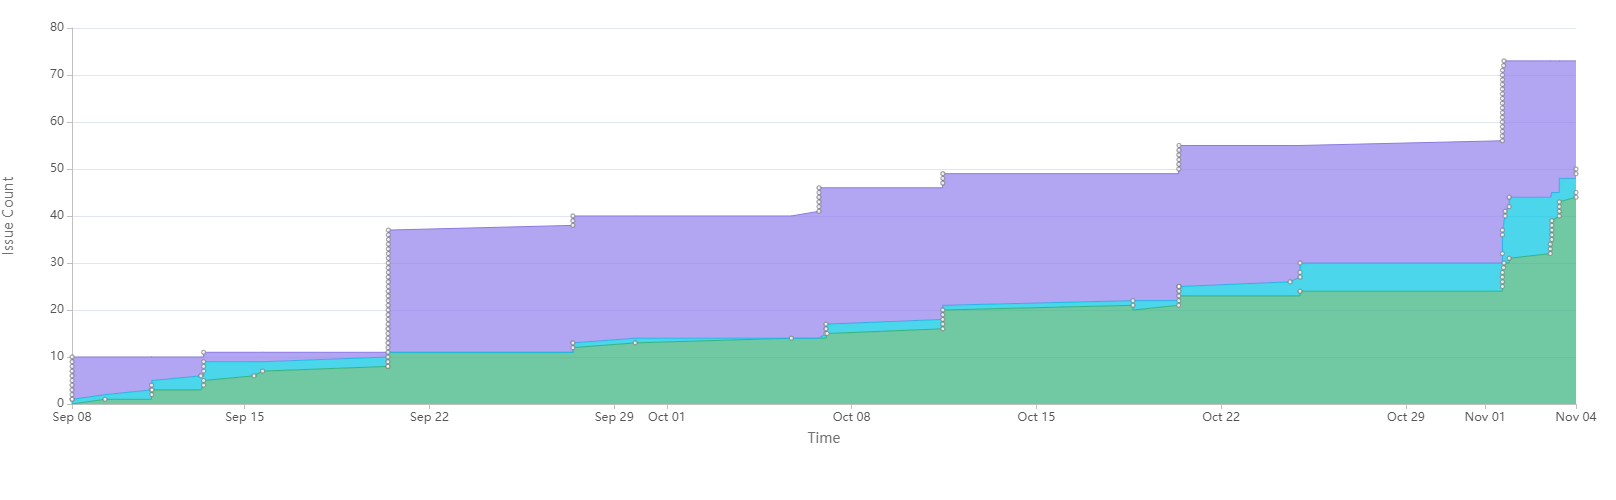
\includegraphics[width=\textwidth]{images/Cumulative flow diagram.png}
    \label{fig:cumulativeflow}
\end{figure}
In Figure \ref{fig:cumulativeflow}: purple designates tasks that are marked unfinished in the the backlog and current sprint, blue represents in progress tasks, and green represents finished tasks.

Throughout Senior Design I we have been gathering research and have started laying out the design of our garden bed and have completed the majority of our part selection. The Figure in \ref{fig:cumulativeflow} may be a little misleading at this point because we have not refined our backlog to fully encapsulate meaningful tasks instead breaking it down into larger subsystem requirement-esque tasks.

